\documentclass[final,t]{beamer}
\catcode`\@=11
\mode<presentation>
{
%  \usetheme{Warsaw}
%  \usetheme{Aachen}
%  \usetheme{Oldi6}
%  \usetheme{I6td}
  \usetheme{I6dv}
%  \usetheme{I6pd}
%  \usetheme{I6pd2}
}



\def\bold#1{\mbox {\bf #1}}\def \vc #1#2{\bold {#1}_{#2}}\def \bftil #1#2{\bold {\widetild #1}_{#2}}
\def\bea{ \begin{eqnarray}}
\def\eea{\end{eqnarray}}
\def\cref#1{(\ref {#1})}
\def\Let@{\relax\iffalse{\fi\let\\=\cr\iffalse}\fi}
\def\vspace@{\def\vspace##1{\noalign{\vskip##1 }}}
\def\mat{\left[\matrix} \def\endmat{\endmatrix\right]}
%\def\vspace@{\def\vspace##1{\noalign{\vskip##1 }}}
\def\matrix{\,\vcenter\bgroup\Let@\vspace@
    \normalbaselines
  \m@th\ialign\bgroup\hfil$##$\hfil&&\quad\hfil$##$\hfil\crcr
    \mathstrut\crcr\noalign{\kern-\baselineskip}}
\def\endmatrix{\crcr\mathstrut\crcr\noalign{\kern-\baselineskip}\egroup
\egroup\,}


% additional settings
\setbeamerfont{itemize}{size=\normalsize}
\setbeamerfont{itemize/enumerate body}{size=\normalsize}
\setbeamerfont{itemize/enumerate subbody}{size=\normalsize}

% additional packages
\usepackage{times}
\usepackage{amsmath,amsthm, amssymb, latexsym,epsfig}
\usepackage{exscale}
%\boldmath
\usepackage{booktabs, array}
%\usepackage{rotating} %sideways environment
\usepackage[english]{babel}
\usepackage[utf8]{inputenc}
\usepackage{natbib}
\usepackage{ragged2e}

\usepackage{subfigure}
\usepackage[orientation=landscape,size=custom,width=90,height=120,scale=1.15]{beamerposter}

\listfiles
\graphicspath{{figures/}}
% Display a grid to help align images
%\beamertemplategridbackground[1cm]



\title{\huge One century of data from Vassouras Magnetic Observatory (1915-2015)}


\author[Benevides et. al.]{Artur Benevides, Edwin Camacho*, Vitor Paes, Rodrigo Melhorato, Israeli Santos and Kátia Pinheiro}
\institute[ON-MCTIC]{Observatório Nacional- ON/MCTIC}
\date[Nov , 2017]{Nov. 15 , 2017}


% abbreviations
\usepackage{xspace}
\makeatletter
\DeclareRobustCommand\onedot{\futurelet\@let@token\@onedot}
\def\@onedot{\ifx\@let@token.\else.\null\fi\xspace}
\def\eg{{e.g}\onedot} \def\Eg{{E.g}\onedot}
\def\ie{{i.e}\onedot} \def\Ie{{I.e}\onedot}
\def\cf{{c.f}\onedot} \def\Cf{{C.f}\onedot}
\def\etc{{etc}\onedot}
\def\vs{{vs}\onedot}
\def\wrt{w.r.t\onedot}
\def\dof{d.o.f\onedot}
\def\etal{{et al}\onedot}
\makeatother

%%%%%%%%%%%%%%%%%%%%%%%%%%%%%%%%%%%%%%%%%%%%%%%%%%%%%%%%%%%%%%%%%%%%%%%%%%%%%%%%%%%%%%%%%%%%%%%%%%%%%%%%%%%%
%%%%%%%%%%%%%%%%%%%%%%%%%%%%%%%%%%%%%%%%%%%%%%%%%%%%%%%%%%%%%%%%%%%%%%%%%%%%%%%%%%%%%%%%%%%%%%%%%%%%%%%%%%%%
\begin{document}

  \begin{columns}[t]
    \begin{column}{.47\linewidth}
%%%%%%%%%%%%%%%%%%%%%%%%%%%%%%%%%%%%%%%%%%%%%%%5 1 !##
\begin{block}{Introduction}
\justifying	
 Vassouras Magnetic Observatory (VSS) was the first observatory in Brazil, starting its measurements in 1915. VSS plays an important role in monitoring of the magnetic field in the south hemisphere mainly because is located in region of Southern Atlantic Magnetic Anomaly (SAMA), in addition, due to its high data quality and transmission in real time VSS is part of the INTERMAGNET (since 1999) network and contributes to development global model.
 
 This work presents the history of VSS as well as the centennial dataset (1915-2015). We	explore the comparison of VSS data and results of IGRF model. We present a solar-quiet (Sq) and storm day to eveluate the influence of the exernal field on VSS and the possible occurrences of the jerks addressing the main characteristics of the secular variation that evidence the variations of internal field.	

\end{block}		

	
	\begin{block}{Theorical Fundamentals}
		
		
		\begin{itemize}
			\item \textbf{Relation between the elements of the geomagnetic field}
		\end{itemize}	
		\[ F^{2} = X^{2} + Y^{2} + Z^{2}, \hspace{1.5cm} H^{2} = X^{2} + Y^{2}, \]
		\[	   X = Hcos(D), \hspace{1.0cm} Y = Hsen(D) \hspace{1.0cm} and \hspace{1.0cm} Z = Fsen(I)\]
	
		
		
		\begin{itemize}	
			\item \textbf{Secular variation}
		\end{itemize}
		The secular variation is the sucessive difference of the values of field components given by:
		\[\frac{dX}{dt} = X(t+1)-X(t)\]
		
		where t represents time in years.
		
		\begin{itemize}
			\item \textbf{Fit by spline interpolation}
		\end{itemize}
		The secular variation of X,Y and Z compontents were fitted using an algorithm  of linear fit by spline method: 
		\[ f(x)= f(x_{n-1})+t_{n-1}(x-x_{n-1}), \\
		for x_{n-1} \le x \le x_{n} \]\\
		
		\begin{itemize}
			\item 	\textbf{Root Means Square (RMS)}
		\end{itemize}
		We calculated the erro between the model IGRF and the data from VSS using RMS:
		\[e_{RMS}=\frac{1}{N} \sqrt{\sum\limits_{i=1}^{N}(VSS_{i}-IGRF_{i})^{2}}, 
		\]
		the RMS can be view in the Table 1.
		
		
	\end{block}	



\begin{block}{Geomagnetic Field Elements}
	\justifying
	
In the figures (1 to 7) below are present the evolution of the main field components over the last 100 years for VSS and IGRF12 model. From 1915 to 1999 the  annual means data  were given directly by VSS, from 1999 to 2015 were performed annual means using the minute data of components from INTERMAGNET. The error RMS between VSS and IGRF can be seen in the Table 1 and the Table 2 shows the rates of change of the Earth's magnetic field  for VSS and IGRF model over the last 100 years.
\\
\end{block}

\begin{columns}

\begin{column}{.49\linewidth}

\begin{block}

\begin{figure}
\centering
\includegraphics[scale=0.6]{"figs_ed/X mean all_V3"}
\caption{1. Annual means: X component}
\label{fig:Xmeanall_V3}
\end{figure}
	
	
\begin{figure}
\centering
\includegraphics[scale=0.6]{"figs_ed/Y mean all_v3"}
\caption{2. Annual means: Y component}
\label{fig:Ymeanall_v3}
\end{figure}

\vspace{0.7cm}

\begin{figure}
\centering
\includegraphics[scale=0.6]{"figs_ed/Z mean all_v3"}
\caption{3. Annual means: Z component}
\label{fig:Zmeanall_v3}
\end{figure}

\vspace{0.7cm}
\begin{figure}
\centering
\includegraphics[scale=0.6]{"figs_ed/F mean all_v3"}
\caption{4. Annual means: F component}
\label{fig:Fmeanall_v3}
\end{figure}

\vspace{0.7cm}
\begin{figure}
\centering
\includegraphics[scale=0.6]{"figs_ed/H mean all_v3"}
\caption{5. Annual means: H component}
\label{fig:Hmeanall_v3}
\end{figure}

	

  
\end{block}	



\end{column}

\begin{column}{.48\linewidth}

\begin{block}

\begin{figure}
\centering
\includegraphics[scale=0.6]{"figs_ed/D mean all_v3"}
\caption{6. Annual means: D component}
\label{fig:Dmeanall_v3}
\end{figure}

\begin{figure}
\centering
\includegraphics[scale=0.6]{"figs_ed/I mean all_v3"}
\caption{7. Annual means: I component}
\label{fig:Imeanall_v3}
\end{figure}

	\begin{table}
		\begin{tabular}{|c|c|}
			\hline
				
			\hline \textbf{Elements}  & \bf{$e_{RMS}}$\\ 
			\hline
			\hline X Component      & 5.23  \\ 
			\hline Y Component     & 12.45\\ 
			\hline Z Component     & 12.67\\ 
			\hline Total field F     & 4.62\\ 
			\hline H      & 3.71\\ 
			\hline Inclination  & 0.03\\ 
			\hline Declination  & 0.03\\ 
			\hline 
		\end{tabular} 
		\vspace{0.5cm}
		\caption{1. Error RMS of the measurements of VSS and IGRF model for the 100 years of data. }
	\end{table}
	
		
	\begin{table}
		\begin{tabular}{|c|c|c|}
			\hline
			\multicolumn{3}{|c|}{\textbf{Change/year}}\\
			\hline	
			\hline   & VSS (nT)& IGRF12 (nT) \\ 
			\hline Total intensity & -22.7  & -3.0 \\ 
			\hline X component & -74.7 & -98.0  \\ 
			\hline Y component & 24.9  & 2.2  \\ 
			\hline Z component & -79.8 & -91.6 \\ 
			\hline H component  & -64.7 & -85.3\\ 
			\hline I component  & $-0^{\circ} 14' 13"$ & $-0^{\circ} 19' 15"$\\ 
			\hline D component  & $-0^{\circ} 7' 2,28"$ & $-0^{\circ} 6' 25"$ \\ 
			\hline 
		\end{tabular} 
		\vspace{0.5cm}
		\caption{2. Change rate for the main field components over 100 years. }
	\end{table}	
\end{block}

\end{column}

\end{columns}




\end{column}
	
\begin{column}{.25\linewidth}
	


\begin{block}{History (1915 - 2015)}
	\justifying	
In 1913 the engineer and director of the Observatório Nacional (ON), Henrique Charles Morize in partnership with the astronomer Alix Correa Lemos idealized the city of Vassouras, RJ (Latitude $22.4 ^{\circ}$ S and $43.35 ^{\circ}$ W) as the ideal place for installation of the VSS, the old place at Morro do Castelo where the Imperial Observatório do Rio de Janeiro (IORJ) was located had a high level of magnetic noise, this problem affects the measurements of the Earth's magnetic field and was the reason for the change of the magnetic observatory from Rio de Janeiro to the Paraíba Valley.  
	
	
	
\end{block}


\begin{block}{Sq and Storm Days}
	\justifying
The Figure below shows the VSS (total field F) for a day with high solar activity, it is observed that near to day 30 of october of 2013 we had a Sq and from there we observed the magnetic storm: 

	\begin{figure}
		\centering
		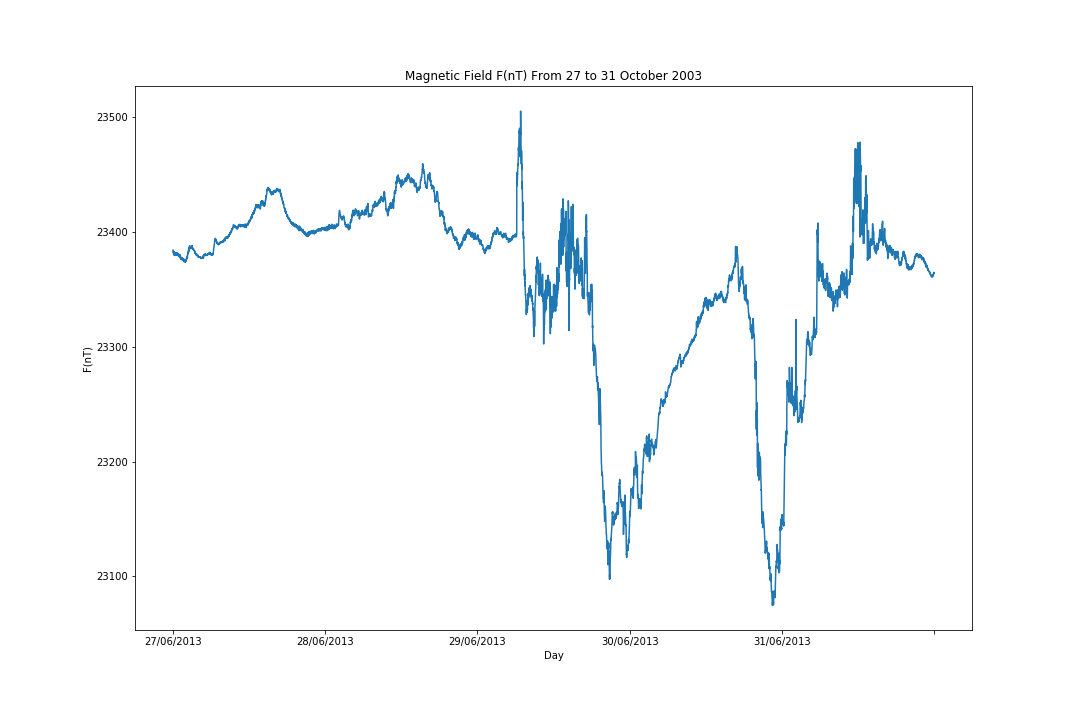
\includegraphics[scale=0.5]{F27_31_october(2003)}
		\caption{8. Storm occurred on October 30, 2013.}
		\label{fig:F27_31_october(2003)}
	\end{figure}
	
	
\end{block}	

	\begin{block}{Geomagnetics Jerks}
		\justifying
		For possibles occurence of jerks we can to analyze first directly the X, Y and Z components using Least Square (LS) to fit trends: 	
		
		\centering
		\begin{figure}
			\centering
			\includegraphics[scale=0.8]{"figs_ed/Linear regression X_v3"}
			\caption{9.For component X, two straight were fitted, showing a trend change and a possible jerk in 1947}
			\label{fig:LinearregressionX_v2}
		\end{figure}
		
		
		\begin{figure}
			\centering
			\includegraphics[scale=0.8]{"figs_ed/Linear regression Y_v3"}
			\caption{10. Possibles jerks occurences in 1937, 1978, 1990 and 2013}
			\label{fintetico}
		\end{figure}	
		
		
		\begin{figure}
			\centering
			\includegraphics[scale=0.8]{"figs_ed/Linear regression Z_v3"}
			\caption{11. Possible jerk occurence in 1965}
			\label{fig:g_Sintetico}
		\end{figure}
		
		
	\end{block}
\end{column}


%%%%%%%%%%%%%%%%%%%%%%%%%%%%%%%%%%%%%%%%%%%%%%%%%%%%%%%%%%%%%%%%%%%%%%%%%%%%%%%%%%%%%%%%%%%%%%%%%%%%%%%%%%%%%%%%%%%

\begin{column}{.25\linewidth}



\begin{block}{VSS}
	\justifying
\begin{figure}
\centering
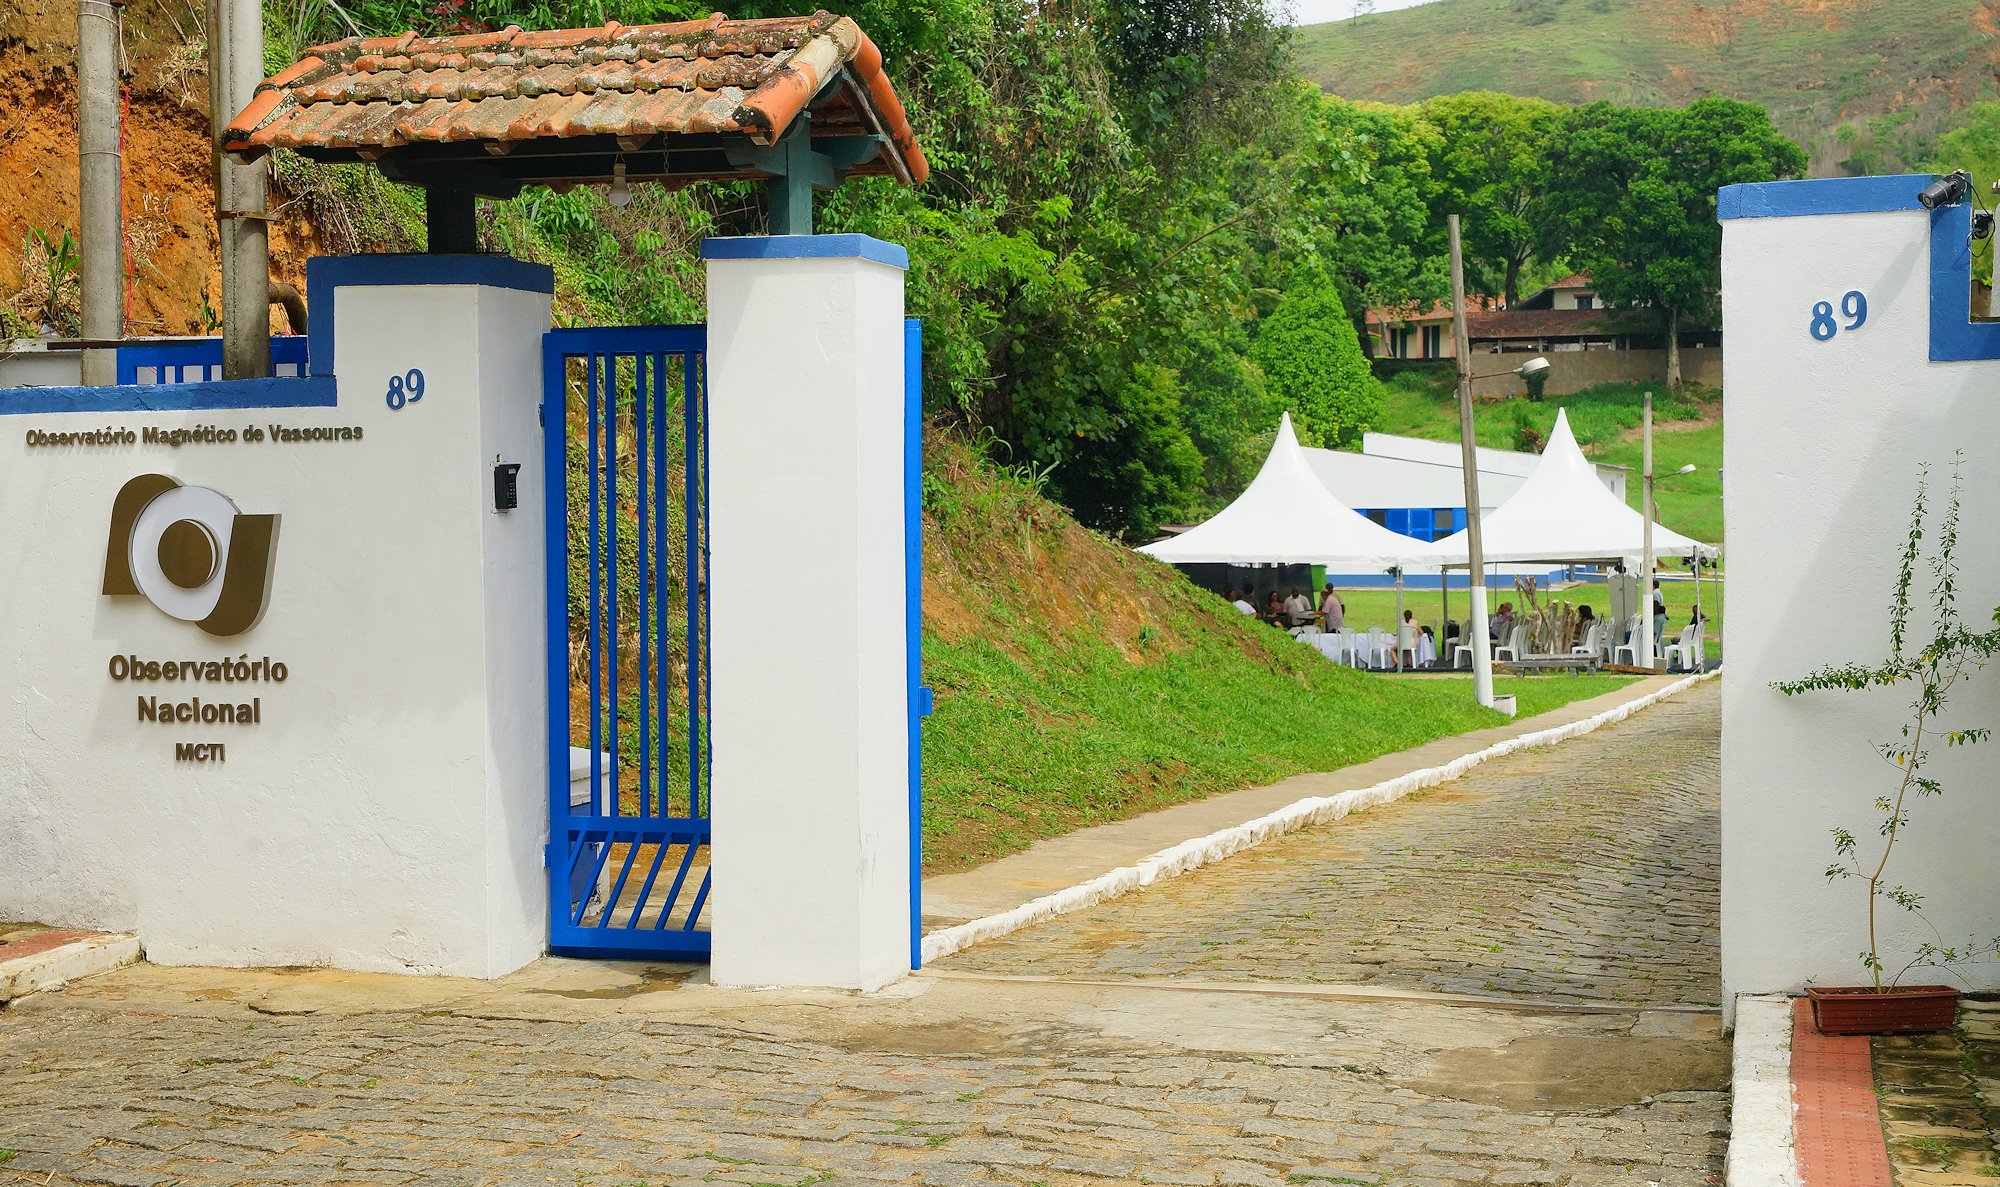
\includegraphics[width=0.9\linewidth]{OMV_JOELSONMOREIRA}
\caption{12. Entrance gate of the Vassouras Magnetic Observatory.}
\label{fig:OMV_JOELSONMOREIRA}
\end{figure}





\end{block}


\begin{block}{VSS}
\centering

	\begin{description}
		\item[\textbf{Period}] | \hspace{0.5cm} Instruments 
				
			\item[\textbf{1915 - 1982}]| Ruska Observatory Pattern (Declination), QHM 534 (Horizontal component) and Earth Inductor Toepfer (Inclination) Variometer unifilar ToepfeR
		\end{description}
	
	 	\begin{description}
	 		\item[\textbf{1982 - 2012}]| DI-flux Bartington, MAG-01 with theodolite Zeiss 010 (1") (Declination and Inclination), PPM Geometrics 816 (Total intensity F).
	 	\end{description}
	
	 
	\begin{description}
		\item[\textbf{2012 - 2014}]| Variometer fluxgate of INTERMAGNET
		
	\end{description}
	
\end{block}



\begin{block}{Geomagnetic Jerks}
Secular variation is widely used to indicate fast changes with time of the main field that are probably due to the changing pattern of core flow	
Analyzing the secular variations (dX/dt, dY/dt e dZ/dt) by spline fits: 		
	\begin{figure}
		\centering
		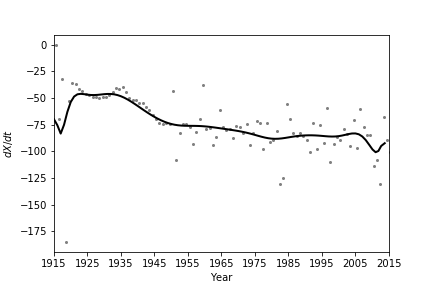
\includegraphics[width=0.8\linewidth]{spline101sv_X_spline}
		\caption{13. Secular variation to X component, possibles jerks: 1935, 1947, 1980, 2005 and 2013}
		\label{SPLINEx}
	\end{figure}
	
	\begin{figure}
		\centering
		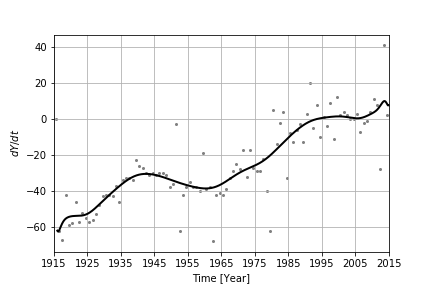
\includegraphics[width=0.8\linewidth]{spline100sv_y_spline}
		\caption{14. Secular variation to Y component, possibles jerks: 1925, 1940, 1960, 1980, 1993 and 2007}
		\label{SPLINEy}
	\end{figure}
	
	\begin{figure}
		\centering
		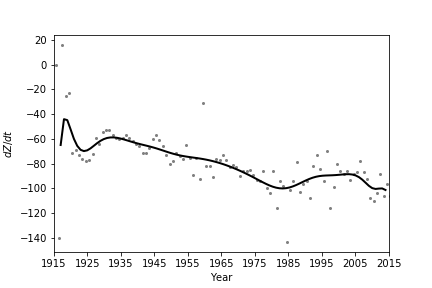
\includegraphics[width=0.8\linewidth]{spline100sv_z_spline}
		\caption{15. Secular variation to Z component, possibles jerks: 1925, 1932, 1983, 2005 and 2013}
		\label{Splinez}
	\end{figure}

\vspace{-0.2cm}
\end{block}

\begin{block}{References}
\begin{itemize}
	\item Observatório magnético de Vassouras: 100 anos de pesquisas e serviçoes prestados à ciências. (2015) Observatório Nacional, Rio de janeiro.
	\item http://www.intermagnet.org

	\item https://www.ngdc.noaa.gov
	
	\end{itemize}


\end{block}

\end{column}

\end{columns}
\end{document}

